\chapter{Introdução\label{cap: intro}}

Apesar de o transporte de cargas e passageiros por meio de veículos guiados datar do século VI~a.C. \cite{lewis_railways_2001} 
e ter sido usado desde então para auxiliar no direcionamento de carroças e vagões por estradas mal conservadas, 
pode-se considerar que o surgimento da ferrovia como uma tecnologia consolidada com a construção da primeira locomotiva a 
vapor pelo engenheiro inglês Richard Trevithick na primeira década do séc.~XIX. Até aquele momento, os vagões ferroviários eram puxados por 
cavalos ou bois, ou funcionavam em sistemas funiculares. Trevithick aperfeiçoou o motor a vapor de água
(trabalho que também vinha sendo conduzido por Nicolas-Joseph Cugnot, considerado o ``pai'' do automóvel) e 
construiu uma máquina de transporte sobre trilhos para demostrar ao público seu invento. Cerca de dez anos depois, 
Matthew Murray produziu uma locomotiva comercialmente viável, corrigindo alguns dos problemas do equipamento de Trevithick, 
e a vendeu para a Middleton Railway \cite{middleton_railway_middleton_2013}, na cidade inglesa de Leeds, dando início 
à indústria de material rodante. 

Nos duzentos anos que se seguiram à demonstração de Trevithick e à máquina de Murray, o trem ganhou todo o mundo. 
A demanda pós-industrial por insumos mais baratos, em grande quantidade e no menor tempo possível, bem como as 
necessidades de deslocamento das pessoas em médias e longas distâncias fez nascer a engenheria ferroviária 
moderna já nas primeiras décadas de 1800. Durante algum tempo as inovações ficaram restritas a minas de 
carvão inglesas, mas logo a colonização do interior dos Estados Unidos, fervilhante logo ao fim da 
Guerra de Independência (1775-1783), e a dinamização das rotas comerciais levou o trem a vapor à 
América, África e Ásia. Os trilhos de madeira foram gradativamente substituídos pelos de aço, mais 
resistentes e confiáveis. Ainda antes da ferrovia moderna, as rodas de veículos ganharam os frisos \cite{wickens_dynamics_1998}, 
de modo a conter os movimentos laterais que 
foram se tornando mais intensos na medida em que a velocidade dos trens aumentava. Os perfis cilíndricos 
originais acabaram substituídos pelo perfis cônicos, devido à estabilidade. As caldeiras 
que alimentavam os grandes motores a vapor primitivos era muito perigosas e a grande quantidade de 
carvão no habitáculo dos funcionários tornava a operação insalubre: foram desenvolvidos grandes propulsores 
Diesel, enormes máquinas elétricas e exerga-se, atualmente, uma tendência ao uso
de células de combustível a base de hidrogênio \cite{ruf_study_2019}. A necessidade de 
velocidade com maior conforto para passageiros aprimorou as suspensões e levou ao desenvolvimento de trilhos e 
fundações de alto desempenho, como as utilizadas hoje em dia nas instalações dos Shinkansen (Japão) e do TGV (França) \cite{iwnicki_future_2009}. 
Como o contato, apesar de todas as melhorias desenvolvidas, ainda é uma fonte de perda, pesquisas com trens de flutuação 
eletromagnética têm avançado, principalmente na Alemanha e no Japão.

No Brasil, o transporte ferroviário moderno chegou em meados do séc.~XIX e se desenvolveu por causa da insistência do Barão de Mauá, 
que financiou a construção da Estrada de Ferro Petrópolis em 1854. A malha ferroviária impulsionou o desenvolvimento das regiões Sudeste e Sul, 
levando trabalhadores da região litorânea para as fazendas de café do interior e retornando com as mercadorias para exportação. 
Foi neste contexto que foram criadas a São Paulo Railway (Jundiaí-Santos) e a Companhia Ferroviária Paulista (Campinas-Jundiaí). 
Durante o governo de D. Pedro II as ferrovias foram utilizadas como um meio de expansão e domínio territorial e no início do 
séc.~XX o país contava com uma das maiores redes do mundo. Devido à grande extensão territorial, a concessão das ferrovias brasileiras 
foi sendo feita de maneira pontual, o que fez com que a mesma estrada passasse sucessiva vezes da iniciativa privada para o governo.
A partir da década de 1950, o movimento de estatização passou a ocorrer com maior intensidade, 
onerando o Governo Federal com a administração da malha. Em 1957 foi criada a Rede Ferroviária Federal (RFF), um órgão de administração 
mista que englobava algumas das principais ferrovias existentes pelo país. 
Alguns anos depois, em 1971, criou-se a Ferrovias Paulistas S.A. (FEPASA) que passou a administrar grande parte da malha paulista que havia sido estatizada. 
Ao fim dos anos 1970 e início dos anos 1980, os investimentos no modal ferroviário foram drasticamente reduzidos, o que levou ao sucateamento parcial da rede,
restando em estado razoável de uso apenas alguns trens metropolitanos e ferrovias ligadas à Companhia Vale do Rio Doce (atual VALE S.A.), 
que transporta ainda hoje grandes quantidades de minério em regiões remotas do Brasil. A partir de 1991, a RFF entrou no plano nacional de estatização, 
por recomendação do BNDES. Em 1998 a FEPASA foi incorporada à autarquia federal e logo em seguida essas empresas foram desmembradas
e seus ramais concedidos para uma série de concessionários, que as administram até o 
presente momento. Quando da privatização das ferrovias, ao final do séc.~XX, os investimentos voltaram a crescer, 
novos projetos foram propostos e o mercado ferroviário acabou por ganhar um novo fôlego. 
A Fig.~\ref{fig: unidades abifer} mostra o número de unidades de vagões de
carga, carros de passageiros e locomotivas entregues por fabricantes nacionais de 1990 a 2020 --  último ano com dados completos publicados.
É observável o aquecimento da produção a partir de 1998, com oscilações consideráveis desde então, mas com valores que
sempre estão bastante superiores aos da década de 1990.

A partir de meados da década de 2010, as operadoras ferroviárias passaram a fazer pedidos de renovação antecipada das
concessões. Tais solicitações ainda não foram todas efetivadas, mas as renovações concedidas até o momento foram condicionadas
a investimentos expressivos nos trechos outorgados. Soma-se a isso um novo modelo de exploração de trechos ferroviários 
por meio de autorizações, de modo que há, quando este texto é escrito, certo otimismo crítico com relação à expansão e revitalização
da malha ferroviária brasileira \cite{rocha_modelo_2022}. 

Atualmente, há no Brasil \SI{30750}{km} de linhas férreas ativas, que pode ser considerado um valor bastante modesto, especialmente ao
se comparar a razão entre extensão da malha ferroviária e área territorial: o país tem \SI{3,61e-3}{\km / \km\squared } (contra valores,
por exemplo, de \num{13,28e-3} e
\num{10,60e-3} de Argentina e México, respectivamente) (ANTF,\citeyear{associacao_nacional_dos_transpotadores_ferroviarios_informacoes_2022}).
Apesar disso, há uma tendência de aumento da malha, discutida no parágrafo anterior, e também da diversificação dos produtos transportados.
Em 1997 para cada 10 toneladas-kilômetro útil (TKU) de minério de ferro transportada do Brasil, apenas \SI{2,4}{TKU} eram transportadas de 
cargas gerais; em 2020, em que pesa a redução geral do transporte devido à pandemia de COVID-19 essa proporção passou para \SI{4,3}{TKU} de
carga geral para cada \SI{10}{TKU} de minério de ferro (ANTF, op.cit.).

\begin{figure}
    \centering
    \begin{tikzpicture}
        \begin{axis}[
            width = \textwidth,
            height=\axisdefaultheight,
            ybar stacked,
            bar width=8pt,
            enlargelimits=0.05,
            legend style={at={(0.5,-0.20)},
              anchor=north,legend columns=-1},
            ylabel={Unidades entregues},
            xtick=data,
            x tick label style={rotate=45,anchor=east},
            ]
        \addplot+[] table [
                    col sep=tab,
                    x=Ano,
                    y=Carros de passageiros,
                ] {Cap_1/Figuras/dados_abifer.dat};
                \addlegendentry{Carros de passageiros}
        \addplot+[] table [
                    col sep=tab,
                    x=Ano,
                    y index=2,
                ] {Cap_1/Figuras/dados_abifer.dat};
                \addlegendentry{Vagões}
        \addplot+[] table [
                    col sep=tab,
                    x=Ano,
                    y index=3,
                ] {Cap_1/Figuras/dados_abifer.dat};
                \addlegendentry{Locomotivas}
        \end{axis}
    \end{tikzpicture}
    \caption{Unidades entregues de carros de passageiros, vagões de carga (geral e minério) e de locomotivas no Brasil desde 1990. Fonte: ABIFER (\citeyear{associacao_brasileira_da_industria_ferroviaria_dados_2022}).}
    \label{fig: unidades abifer}
\end{figure}

\section{Simulação de veículos ferroviários}
Os princípios matemáticos que regem o comportamento dos veículos ferroviários vêm sendo estudados desde o
início da indústria ferroviária. Atribui-se a George Stephenson a ideia de utilizar perfis cônicos para melhorar
a estabilidade -- especialmente de locomotivas \cite{wickens_dynamics_1998, knothe_rail_2017}. \citeonline{redtenbacher_gesetze_1855} 
formulou matematicamente o problema das rodas cônicas realizando curvas e também propôs o primeiro modelo de contato conforme, isto é,
que inclui a deformação das superfícies \cite{knothe_history_2008}. Apenas alguns anos mais tarde, \citeonline{hertz_ueber_1882} desenvolveria
sua teoria sobre contato de corpos elásticos, considerando, então, limites de elasticidade para determinar a deformação. Redtenbacher, portanto,
não possuía ainda as ferramentas teóricas para aprimorar seu modelo de contato roda trilho, mas conseguiu explicar o surgimento
básico das oscilações cinemáticas que ocorrem nos rodeiros com rodas cônicas.

\begin{figure}
    \centering
    \begin{tikzpicture}
        \pic[rotate=1, transform shape, shift={(0.1,0)}]{rodeiro};
        \draw[rotate = 1,cota] (-3.45,0) -- +(0,-2.02) node [midway, fill=white] {$R_l$};
        \draw[rotate = 1,cota] (3.36,0) -- +(0,-2.18) node [midway, fill=white] {$R_l$};
        \pic[rotate=-1.43,scale=0.2,shift={(-18,-18.2)}]{trilho};
        \pic[rotate=1.43,scale=0.2,shift={(18,-18.2)}]{trilho};
        \draw[thick, -stealth] (0,-2) -- +(1,0) node [anchor=west] {$y_t$};
        \draw[thick, -stealth] (0,-2) -- +(0,-1) node [anchor=west] {$z_t$};
    \end{tikzpicture}
    \caption{Rodeiro ferroviário deslocado do centro da via.}
    \label{fig: rodeiro ferroviario desloc}
\end{figure}

As \textit{oscilações cinemáticas} apontadas por Redtenbacher são associadas, mas não descrevem completamente, o fenômeno
de \textit{hunting} que ocorre em veículos ferroviários. A ideia fundamental é que se um rodeiro que anda em linha reta, no
sentido do eixo $x_t$ da Fig.~\ref{fig: rodeiro ferroviario desloc}, mas em algum momento é deslocado lateralmente no sentido
positivo de $y_t$, então os raios de rotação das rodas esquerda $R_l$ e direita $R_r$ alteram-se de modo que o primeiro diminui
e o segundo aumenta de um fator $\Delta R$. Como ambas as rodas são solidárias ao eixo do rodeiro, elas precisam ter a mesma
velocidade angular ao redor desse eixo, de modo que o ponto de contato com o trilho da roda da direita move-se mais rápido do que o ponto de 
contato com o trilho da esquerda. Assim, induz-se no rodeiro um movimento de guinada (rotação ao redor do eixo vertical $z_t$),
que por sua vez aumenta o raio de contato da roda esquerda e reduz da direita, invertendo o sentido da diferença de velocidades
dos pontos de contato. Isso produz um movimento oscilatório combinado de deslocamento lateral e guinada do rodeiro.

Conforme citado em diversas fontes, como \citeonline{knothe_rail_2017}, \citeonline{wickens_dynamics_1998} e \citeonline{shabana_railroad_2008},
foi Johann Klingel quem primeiro desenvolveu uma solução analítica para as oscilações cinemáticas descritas por Stephenson e Redtenbacher, 
em um artigo de 1883 intitulado \textit{Über den Lauf von Eisenbahnwagen auf gerader Bahn} (``Sobre o movimento de veículos ferroviários em 
linha reta'' em uma tradução livre). Klingel obteve, para o problema do deslocamento lateral do rodeiro durante a oscilação cinemática,
uma equação diferencial de segunda ordem, não amortecida. A partir disso, estabeleceu o comprimento de onda característico $\Lambda$ da vibração do
rodeiro como sendo:

\begin{equation}
    \Lambda = 2\pi \left(\frac{R_0 b}{2\lambda}\right)^{1/2}
    \label{eq: klingel}
\end{equation}
onde $R_0$ é o raio de rolamento nominal da roda, $b$ é a bitola de contato, isto é, a distância lateral entre os pontos de contato roda-trilho
do mesmo rodeiro, e $\lambda$ é a conicidade das rodas.

Como se pode observar, a Eq.~\eqref{eq: klingel} mostra que o comprimento de onda da oscilação depende unicamente de parâmetros geométricos e que,
portanto, a frequência do movimento cresce linearmente com a velocidade de translação. Como aponta \citeonline{wickens_dynamics_1998}, não há muito mais que possa 
ser deduzido sobre o movimento a partir das conclusões de Klingel. Principalmente, a solução de Klingel aponta para uma solução estacionária da oscilação,
que não cresce nem decresce ao longo do tempo. Já no séc.~XIX, no entanto, já se sabia que sob certas condições o movimento dos rodeiros poderia tornar-se
instável, sendo limitado apenas pelas flanges.

\begin{figure}
    \centering
    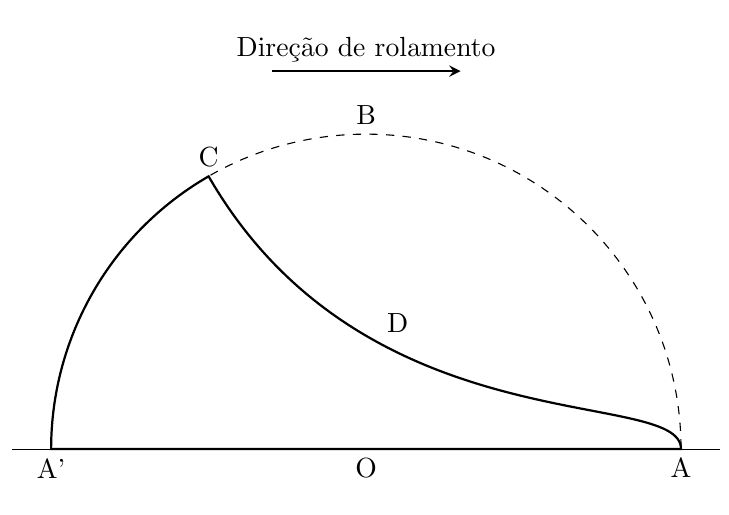
\begin{tikzpicture}[scale=0.4,out=45,in=135,distance=1cm]
        \draw[shorten <= -5mm,shorten >= -5mm] (-10,0) node [anchor=north]{A'} -- (10,0) node [anchor=north] {A} node [midway, anchor=north] {O};
        \draw[dashed] (-10,0) arc (180:0:10) node[midway, anchor=south] {B};
        \draw[thick] (-10,0) arc (180:120:10) node[above] {C} to [controls=+(-60:10) and +(90:2)] (10,0) -- cycle;
        \node (D) at (1,4) {D};
        \draw[thick,-stealth] (-3,12) -- (3,12) node[midway, anchor=south] {Direção de rolamento};
    \end{tikzpicture}
    \caption{Curva de escorregamento da região de contato proposta por \citeonline{carter_action_1926}. A linha $AA'$ representa
    a região de contato e o eixo vertical é o limite de aderência de atrito na roda. No trecho $ADC$ roda e trilho estão aderidos e
    as forças de atrito (\textit{creepage}) apenas equilibram as tensões de cisalhamento. No trecho $CA'$ a tensão de cisalhamento
    é muito elevada, o que causa escorregamento local das superfícies.}
    \label{fig: creep carter}
\end{figure}

Foi \citeauthor{carter_electric_1916} (\citeyear{carter_electric_1916,carter_action_1926}) quem percebeu que a formulação do fenômeno de 
oscilações cinemáticas dos rodeiros ferroviários só poderia
estar completa com a descrição adequada não só da cinemática, mas também das forças de contato entre rodas e trilhos. Ele introduziu a ideia de 
\textit{creep}, ou escorregamento, que é uma consequência das deformações elásticas dos materiais de roda e trilho ao redor da região de 
contato (Fig.~\ref{fig: creep carter}). 
Os resultados de \citeauthor{carter_electric_1916} e de \apudonline{boedecker_wirkungen_1887}{knothe_history_2008} -- que propusera um modelo
de contato baseado no atrito de Coulomb -- comprovaram que o movimento oscilatório dos rodeiros é inerentemente instável, sendo sempre limitado pelas flanges.
A instabilidade, no entanto, poderia ser evitada se os rodeiros fossem montados em suporte flexível com propriedades adequadas de rigidez (esse é
o papel das suspensões secundárias modernas), como mostrou, anos mais tarde, Matsudaira, cujo trabalho fora inicialmente publicado apenas em japonês
e, em 1960, entrou em um relatório do Comitê C9 do ORE (\textit{Office de Recherche et d'Essais de l'Union International des Chemins de Fer}) \apud{matsudaira_shimmy_1952}{wickens_dynamics_1998,gilchrist_long_1998,knothe_rail_2017,iwnicki_handbook_2006}. 
\citeonline{wickens_dynamics_1965} apurou o desenvolvimento de Matsudaira com base em modelos computacionais e testes
de bacada conduzidos no Reino Unido. Foi Wickens quem introduziu a ideia de elementos de amortecimento das vibrações laterais dos rodeiros.

Aqui cabe uma observação sobre um termo que surgiu anteriormente. Há alguns parágrafos, afirmou-se que as considerações de \citeauthor{redtenbacher_gesetze_1855}
não explicavam totalmente o fenômeno de \textit{hunting} que, em termos observacionais, é justamente a oscilação
combinada de movimentos laterais e de guinada do rodeiro. Com o modelo de \textit{creep} proposto por \citeauthor{carter_electric_1916}
e as análises de estabilidade conduzidas por \citeauthor{matsudaira_shimmy_1952} e \citeauthor{wickens_dynamics_1965}, finalmente o \textit{hunting}
foi percebido como um tipo de oscilação auto-excitada, causada por um distúrbio da condição de equilíbrio lateral do sistema 
rodeiro-trilho, sujeita a zonas de instabilidade e à formação de ciclos-limite. Deste ponto do texto para frente, o termo \textit{hunting}
será utilizado para designar o fenômeno da oscilação lateral e de guinada do rodeiro, com características de instabilidade.
 
\citeonline{evans_challenges_2009} apontam a década de 1960 como o início da dinâmica ferroviária como tema de estudo acadêmico, 
graças, em grande parte, às contribuições dos autores citados nos parágrafos anteriores. Os próximos grandes passos em direção ao
uso generalizado de ferramentas de simulação para o projeto de veículos ferroviários seriam dados por \citeauthor{johnson_effect_1958}, Vermeulen
e \citeauthor{kalker_rolling_1967}.

\citeonline{johnson_effect_1958} propôs, pela primeira vez, uma solução para o problema de contato com rolamento entre dois corpos.
É importante ressaltar que a teoria de contato de \opcit{hertz_ueber_1882} resolvia o contato estático entre corpos elásticos, o
que não incluía as tensões tangenciais causadas por atrito. \citeonline{kalker_rolling_1967}, por sua vez, criou uma implementação
computacional para solucionar as equações de contato entre corpos em movimento. Para tanto, Kalker assumiu que a área de contato
seria elíptica e utilizou uma abordagem por elementos de contorno. Além disso, adicionou um momento de resistência ao deslizamento (\textit{spin}). 
Em sua tese de doutorado, de \citeyear{kalker_rolling_1967},
Kalker introduziu o que se conhece atualmente por \textit{teoria linear}, que assume que o deslizamento real entre trilho e roda
é zero em toda a área de contato. O termo
\textit{deslizamento real} refere-se à combinação do deslizamento de corpo rígido (sem deformação) entre roda e trilho, mais o
deslizamento devido à deformação dos materiais em contato. A teoria linear utiliza o que se conhece por coeficientes
de Kalker para estabelecer uma relação linear entre os escorregamentos e as forças de contato tangenciais.

A rigor, a apresentação que Kalker fez inicialmente da teoria de contato com rolamento é bastante genérica, considerando inclusive
os parâmetros dos materiais para as equações. A solução linear, então, já era uma simplificação de um modelo mais geral. Algum tempo depois
\apud{kalker_simplified_1973}{zaazaa_review_2009}, o próprio Kalker apresentou sua teoria simplificada, que assume uma relação linear
entre as forças lateral e longitudinal e os escorregamentos nas respectivas direções. Também considera que a força de tração vai a zero no 
bordo de ataque da região de contato. A teoria simplificada deu origem ao algoritmo FASTSIM, que ainda hoje é muito utilizado em 
programação de simulação ferroviária, pois suas respostas são bastante aderentes aos resultados experimentais para uma boa parte
das aplicações.

Na década de 1980, \citeauthor{kalker_principle_1986} expandiu os modelos simplificados ao abandonar a hipótese de área elíptica de contato e ao formular os 
deslizamentos como funções dos parâmetros dos materiais. Esse desenvolvimento só foi possível devido ao avanço da computação, pois
a solução das equações obtidas de maneira adequada exige bastante poder de processamento. O programa CONTACT foi desenvolvido com base
na teoria completa do contato tridimensional e continua sendo mantido até hoje.

Atualmente, existem diversos pacotes computacionais capazes de simular um veículo ferroviários em diferentes níveis de complexidade. Entre eles, é possível fazer duas grandes divisões entre \textit{software} dedicados e de uso geral:
\begin{itemize}
 \item \textbf{Dedicados:} foram desenvolvidos para simulação de veículos ferroviários e, por isso, possuem características voltadas para a engenharia ferroviária, como elementos de suspensão, mancais, trilho etc. Os programas NUCARS, Vampire, GENSYS e Universal Mechanism (apesar de o último também contar com um módulo de uso geral) são exemplos conhecidos. Os dois primeiros, em particular, são bastante utilizados na indústria;
 \item \textbf{Uso geral:} são, na verdade, programas multicorpos para simulação de mecanismos que foram, ao longo do tempo, sendo adaptados para soluções específicas. Os dois representantes comerciais mais comuns são o MSC/ADAMS e o SIMPACK.
\end{itemize}
Com a popularização dos programas de código aberto, algumas soluções colaborativas de sistemas multicorpos podem ser adaptadas para o uso específico da simulação ferroviária. O MBSim \cite{schindler_analysing_2010}, desenvolvido pela Universidade Técnica de Munique, o MBDyn, do Politécnico de Milão, e o HOTINT, que é mantido pela Linz Center of Mechatronics GmbH (empresa filha da Universidade Johannes Kepler de Linz, na Áustria).

Assim como ocorre em outras áreas ligadas à tecnologia da mobilidade, o uso de modelos computacionais no contexto da engenharia ferroviária tem como objetivos principais reduzir custos, tempo de projeto e melhorar a capacidade de predição do comportamento dos sistemas, já que as modificações durante o processo de desenvolvimento do produto podem ser testadas de maneira virtual. De fato, ao longo dos últimos anos trabalhos de simulação auxiliaram na definição, por exemplo, de novos perfis de roda, soluções de suspensão e métodos de fixação dos trilhos. O conceito de \textit{gêmeos digitais}, associado ao programa de manufatura avançada promovido pelo governo alemão desde o início da década de 2010, prevê o uso de modelos matemáticos rápidos, mas realistas, para analisar em tempo real dados provenientes de sensores. A implementação dessa técnica para ferrovias passa, obrigatoriamente, pelo uso de simulações multicorpos eficientes que possam representar de maneira fidedigna as condições da operação ferroviária \cite{dimitrova_digital_2021,errandonea_iot_2021}.

\section{Objetivos do trabalho}
Este trabalho busca preencher algumas lacunas ainda abertas no tema de simulação computacional de veículos ferroviários. Os avanços nesse campo ao longo dos últimos anos foi considerável, mas há certos tópicos que a comunidade científica \cite{evans_challenges_2009} julga serem interessantes:
\begin{itemize}
 \item \textbf{Modelos mais precisos para contato roda-trilho}. Apesar das conquistas promovidas por Kalker e outros, diversos fenômenos que ocorrem na região de contato da roda com o trilho ainda não são plenamente compreendidos, como: efeitos de alta frequência, adição de modificadores de atrito, desgaste e fadiga de rodas;
 \item \textbf{Métodos de solução das equações de movimento}. Como se verá ao longo deste texto, as equações de movimento de um sistema ferroviário são bastante complexas e não lineares, especialmente devido à necessidade de se considerar os contatos e suas implicações não holonômicas;
 \item \textbf{Modelos mais detalhados para a dinâmica da via}. É um tema de grande relevância, pois é da via que vem a maioria das excitações dos veículos. Devido à complexidade da interação entre o veículo e os trilhos, os modelos mais populares são resultado de simplificações que podem mascarar alguns efeitos.
\end{itemize}

É sobre esse último item que este trabalho se debruça. Os modelos matemáticos de interação veículo-via atualmente utilizados ora utilizam uma via excessivamente simplificada - modelos de pista rígida, ou de massas concentradas ligadas por molas -, ora um veículo excessivamente simplificado - apenas um rodeiro em contato com os trilhos. Já é fato estabelecido que a consideração da flexibilidade da via tem papel importante na avaliação da dinâmica veicular em frequências superiores a \SI{200}{\hertz}, como apontam, entre outros, \citeonline{knothe_rail_2017,popp_combined_2003} e \citeonline{guimaraes_alise_1999}. As abordagens para esse problema, que serão discutidas com mais profundidade no 
Cap.~\ref{cap: revisao}, incluem modelos com elementos discretos de trilho apoiados sobre conjuntos de molas e amortecedores \cite[p.26]{knothe_rail_2017}, linearizações para uso 
em análises no domínio da frequência \cite{ding_effects_2016}, redução modal a partir de modelos de elementos finitos \cite{baeza_railway_2011}, uso apenas de elementos finitos \cite{guimaraes_alise_1999,lundqvist_load_2005}, co-simulação entre códigos multicorpos e de elementos finitos \cite{pombo_flexible_2013,pombo_development_2019} e implementação direta de elementos finitos em algoritmos multicorpos \cite{shabana_absolute_1997,shabana_alternative_2009}.

O presente estudo, então, tem dois pontos focais: (a) propor um modelo dinâmico de interação veículo-via que apresente um vagão com suspensão completa (primária, secundária, inércias rotativas) apoiado sobre uma via permanente flexível, usando uma abordagem por dinâmica multicorpos acoplada diretamente com elementos finitos e (b) investigar os efeitos do acoplamento da flexibilidade da via com os movimentos induzidos no vagão. De maneira particular, destaca-se, aqui, o estudo de vagões de carga, que tem sido menos explorados na literatura com respeito à interação com via flexível. Com isso, pretende-se fazer uma contribuição ao estudo da interação entre veículos ferroviários e vias flexíveis.

\section{Organização do documento}